% ----------------------------------------------------------------
% Revisão bibliográfica *******************
% ----------------------------------------------------------------
\chapter{Metodologia}
\label{cap:revisao}
%
%
\section{O software Tiled}
\label{tiled}
%
A grande maioria dos jogos eletrônicos 2D apresenta, além dos \textit{sprites} dos personagens e itens, uma imagem representando o cenário do jogo. Dependendo da natureza do jogo, esses cenários podem possuir grandes dimensões, o que torna custoso para o software do jogo carregar e 
armazenar essa imagem em memória (RAM e em disco). Mas, se analisarmos a imagem que representa o cenário, vamos verificar que o mesmo é formado
por pequenas partes que se repetem com muita frequência. Assim, aproveitando dessa característica e com o objetivo de diminuir o consumo de
memória e o desempenho ao carregar imagens de resolução elevada, foi desenvolvida uma técnica conhecida como \textit{TileMap}. A técnica
consiste no uso de uma imagem, chamada \textit{tileset}, contendo pequenos pedaços de imagens, conhecidos como \textit{tiles}, que são
as imagens que se repetem em grande quantidade na imagem do cenário de jogo. Estes \textit{tiles} são usados 
para criar uma imagem composta denominada \textit{tiled layer}.
%
%
\begin{figure}[H]
    \centering
    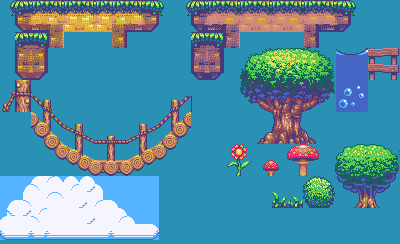
\includegraphics[scale = 1.0]{Imagens/tileset_edit.png}
    \caption{\textit{Exemplo de \textit{tileset}.}}
    \label{tileset_example}
\end{figure}
%
\par
%
O cenário final do jogo pode ser constituído de um único \textit{tiled layer} ou ser resultante da combinação 
de dois ou mais \textit{tiled layers}. Através da técnica de \textit{Tilemap}, torna-se possível construir inúmeros cenários,
com variadas dimensões, usando como base o mesmo \textit{tilesets}, aumentando a economia de memória e não reduzindo o desempenho 
no carregamento de imagens.
%
%
%
\begin{figure}[H]
    \centering
    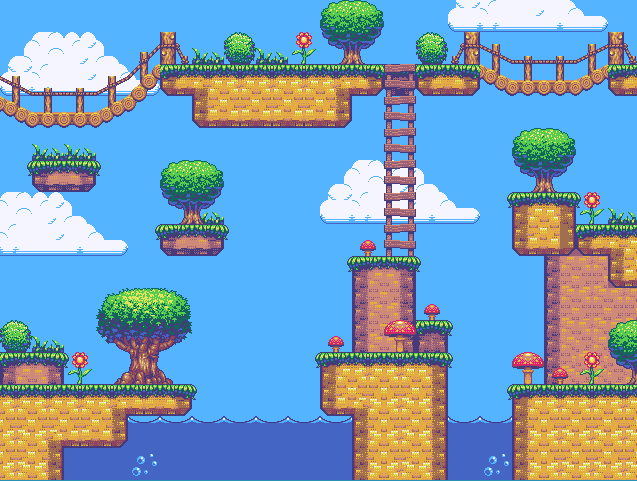
\includegraphics[scale = 0.65]{Imagens/cenario.png}
    \caption{\textit{Exemplo de um cenário construído com tileset.}}
    \label{cenario_example}
\end{figure}
%
%
\par
O software Tiled \cite{SiteTiled} é uma ferramenta gratuita desenvolvida em C++ para a criação de layouts e mapas usando \textit{tilesets}
baseado na técnica de \textit{Tilemap}. De simples manuseio e grande versatilidade, o Tiled faz a edição de várias camadas 
de \textit{tiles} e salva tudo em um formato padronizado de extensão ``.tmx''. Uma das principais vantagens do formato TMX é sua organização, 
detalhamento e praticidade, sendo que seu conteúdo pode ser lido através do uso de um \textit{parser} para arquivos XML.
%
\begin{figure}[H]
    \centering
    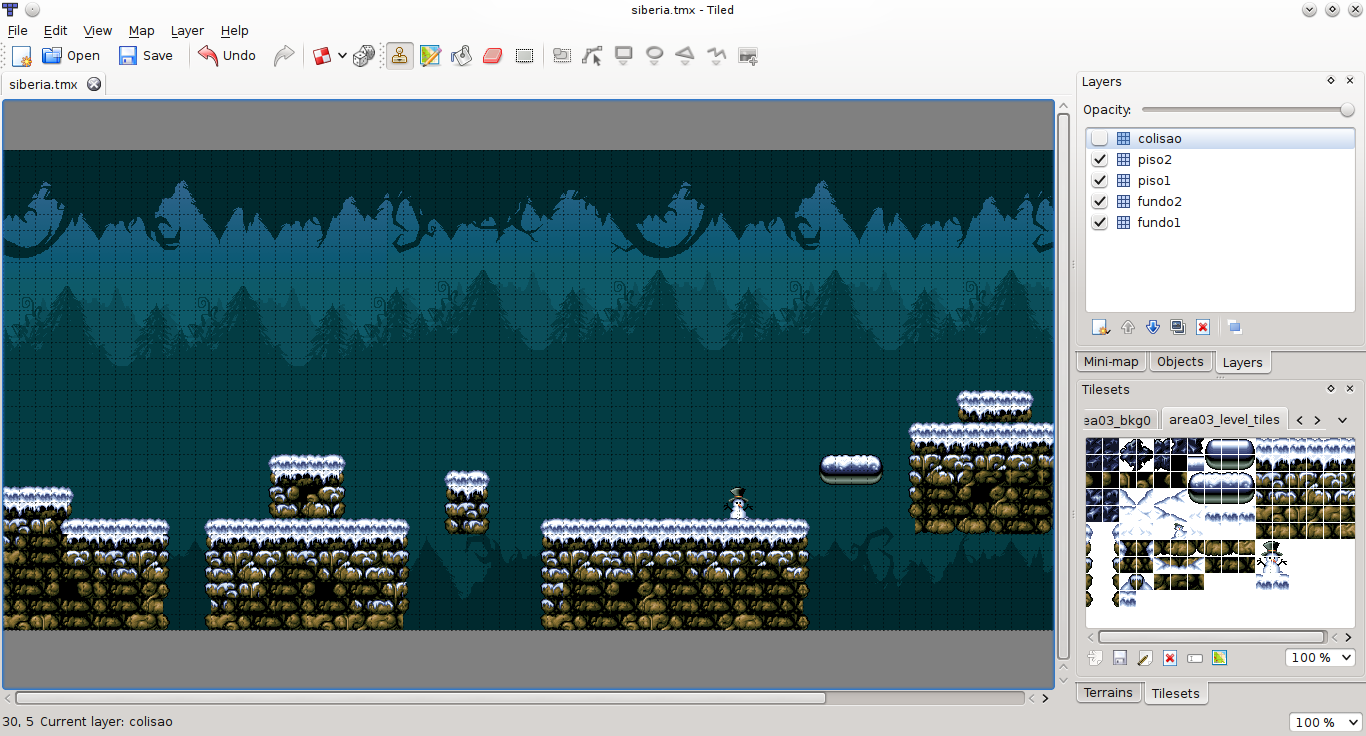
\includegraphics[scale = 0.45]{Imagens/Tiled.png}
    \caption{\textit{Interface do \textit{software} Tiled.}}
    \label{tiled_interface}
\end{figure}
%
\par
O Tiled é um editor de níveis que suporta mapas com projeções ortogonais e isométricas e ainda permite que 
objetos personalizados sejam salvos como imagens na resolução que desejar. Tem suporte também a comandos externos, 
\textit{plugins} e formatos usados por outros editores. É compatível 
com diversas \textit{engines} de criação de jogos e fornece meios de comprimir seus dados de modo a diminuir o tamanho em disco do arquivo TMX.
É possível, ainda, redimensionar e alterar o mapa posteriormente, criar múltiplos mapas em uma única sessão e ainda salvar ou 
restaurar até nove vezes. Com ele pode-se especificar o tamanho de cada \textit{tile} em um \textit{tileset}, ou criar um mapa sem tamanho estrito 
sobre as imagens \cite{TiledTutorial}.
Mesmo que o desenvolvedor não queira que seu jogo seja baseado em \textit{tiles}, o software é ainda uma excelente escolha como um editor 
de níveis. Pode-se usá-lo também nas entidades invisíveis, tais como áreas de colisão e o aparecimento de objetos dentro do 
mapa. Por sua simplicidade ela pode ser usada por programadores iniciantes ou experientes.
\par 
O processo de criação de um mapa com o Tiled é feito basicamente usando os passos abaixo:
%
\begin{enumerate}
 \item Escolher o tamanho do mapa e tamanho do \textit{tile} base;
 \item Adicionar \textit{tilesets} vindos de imagens;
 \item Adicionar quaisquer objetos que representem algo abstrato;
 \item Salvar o mapa no format TMX;
 \item Importar o arquivo TMX e interpretá-lo para o jogo.
\end{enumerate}
%%
O Tiled é totalmente gratuito. Esse detalhe aliado à sua facilidade de uso e versatilidade, tornaram-no extremamente popular em meio
à comunidade de desenvolvedores de jogos, onde não só estudantes e entusiastas, mas também empresas e profissionais da área, passaram a adotá-lo 
como editor de níveis padrão. Seguindo esse pensamento, o nosso \textit{framework} a ser desenvolvido também possui suporte nativo
aos níveis construídos usando esse software.
%
%
%

%
%

